\documentclass{article}

%Packages
\usepackage{graphicx}

%Standart stuff
\title{Status Quo der digitalen Gesundheitsanwendungen}
\author{Marcelo Hauger}
\date{\today}

\begin{document}
	\maketitle
	\newpage
	\tableofcontents
	\newpage
	\section{Grundlagen}
		Durch das Inkrafttreten des Digitale-Versorgung-Gesetzes (DVG) am 19. Dezember 2019 wurden Digitale Gesundheitsanwendungen für Patienten in die Gesundheitsversorgung eingeführt (§§ 33a und 139e Fünftes Buch Sozialgesetzbuch). Ungefähr 73 Millionen Versicherte in der gesetzlichen Krankenversicherung haben Anspruch auf DiGA-Versorgung, die von Ärzten und Psychotherapeuten verordnet und von der Krankenkasse erstattet werden können.
		\subsection{Was ist eine "DiGA"?}
			DiGA (Digitale Gesundheitsanwendung), als "digitale Helfer" in der Hand der Patientinnen und Patienten, bieten zahlreiche Möglichkeiten, Krankheiten zu erkennen und zu behandeln sowie den Weg zu einer selbstbestimmten, gesundheitsförderlichen Lebensführung zu unterstützen. Die DiGA müssen als CE-gekennzeichnetes Medizinprodukt folgende Eigenschaften mit sich bringen:
			\begin{itemize}
				\item Ein Medizinprodukt der Risikoklasse 1 oder 2a nach MDR (Medical Device Regulation) und im Rahmen der Übergangsvorschriften nach MDD (Medical Device Directive).
				\item Die Hauptfunktion basiert auf digitalen Technologien.
				\item Der medizinische Zweck wird wesentlich durch die digitale Hauptfunktion erreicht.
				\item Die DiGA unterstützt die Erkennung, Überwachung, Behandlung oder Linderung von Krankheiten oder die Erkennung, Behandlung, Linderung oder Kompensierung von Verletzungen oder Behinderungen.
				\item Die DiGA wird entweder vom Patienten, oder vom Leistungserbringer und Patient gemeinsam genutzt.
			\end{itemize}  
			Diese Anforderungen sind in § 33a Fünftes Buch Sozialgesetzbuch (SGB V) definiert.\cite[vgl. Was ist eine DiGA?]{wissenswertes-diga}
		\newpage
		\subsection{Fast-Track-Verfahren} 
			\begin{figure}[htbp]
				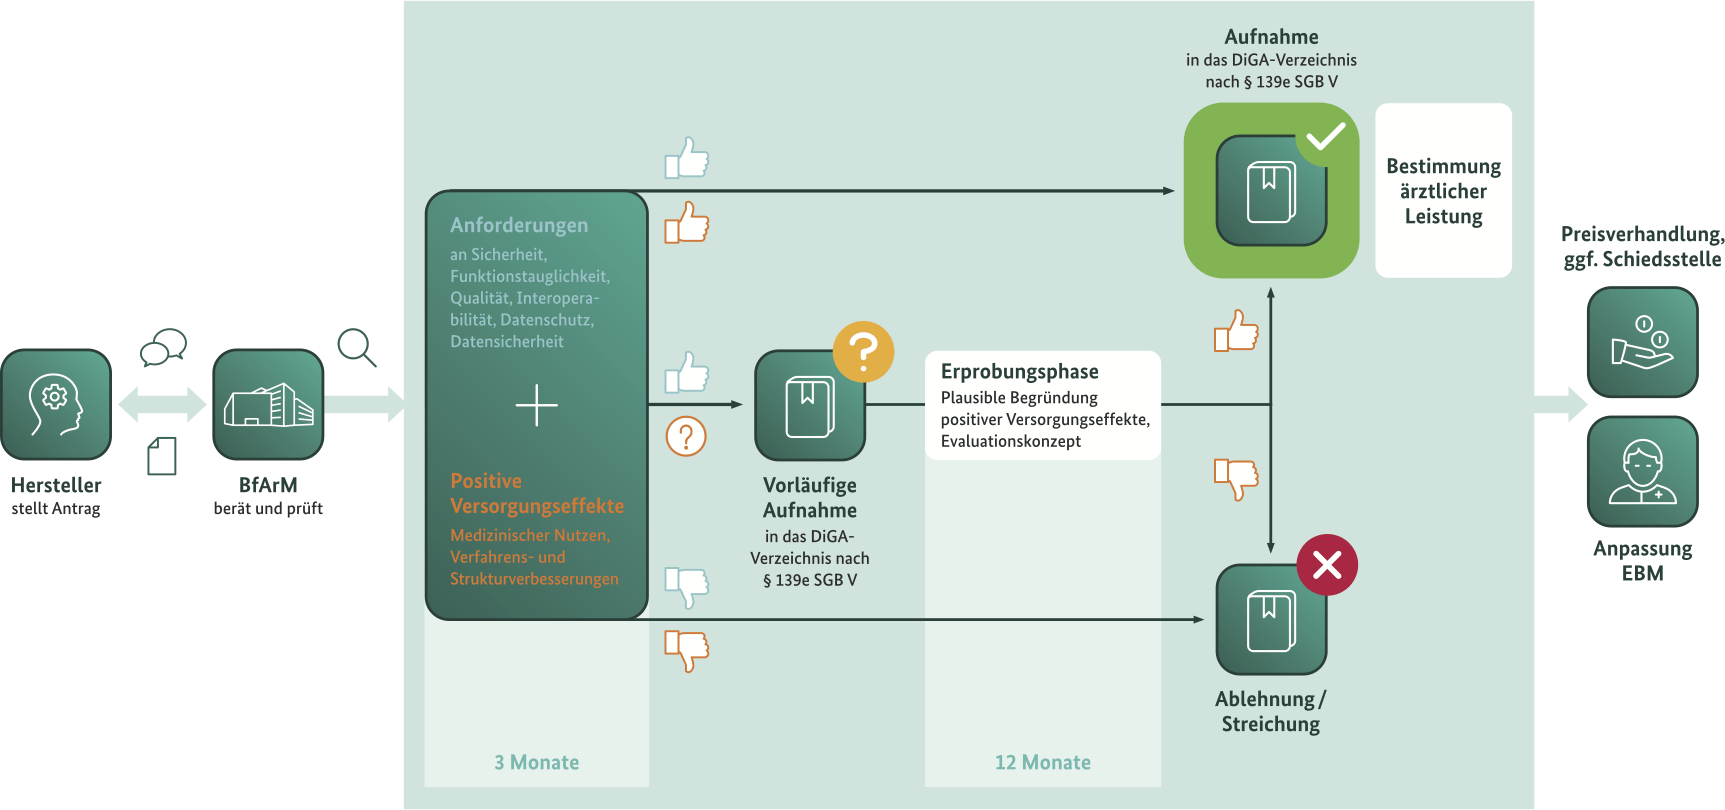
\includegraphics[width=\textwidth]{./grafiken/fast-track-verfahren}
				\caption[Ablaufdiagramm des Fast-Track-Verfahren]{Ablaufdiagramm des Fast-Track-Verfahren}
				\label{Abb-ft-Verfahren}
			\end{figure}
			In der Abbildung wird das am 27. Mai 2020 entstandene Fast-Track-Verfahren beschrieben. Im Türkisen Bereich der Abbildung sieht man, wie das Fast-Track-Verfahren abläuft. Im grünen Kasten, auf der linken Seite des Türkisen Bereichs, sieht man die 2 Voraussetzungen für eine erfolgreiche Antragsstellung die über 3 Monate hinweg vom Bundesinstitut für Arzneimittel und Medizinprodukte. Dabei gibt es die technischen Anforderungen, wie: Sicherheit, Qualität, Datenschutz etc. und die Positiven Versorgungseffekte: Medizinischer Nutzen, Verfahrens- und Strukturverbesserungen. Sollten beide Voraussetzungen erfüllt sein, wird der Antrag akzeptiert und es kommt zu Preisverhandlungen, wie man rechts oben im Türkisen Bereich sehen kann. Sollten beide Voraussetzungen nicht erfüllt sein, wird der Antrag abgelehnt, wie man rechts unten im Türkisen Bereich sehen kann. Sollten nun die technischen Anforderungen erfüllt sein, aber der Positive Versorgungseffekt noch fragwürdig sein, wird die DiGA vorläufig aufgenommen und es kommt zu einer 12-Monatigen Erprobungsphase.
		\newpage
	\section{Informationen zu den DiGAs}   
		Im folgenden Kapitel werden allgemeine Informationen zu den DiGA wiedergegeben.
		\subsection{Fast-Track-Verfahren} 
			\begin{figure}[htbp]
				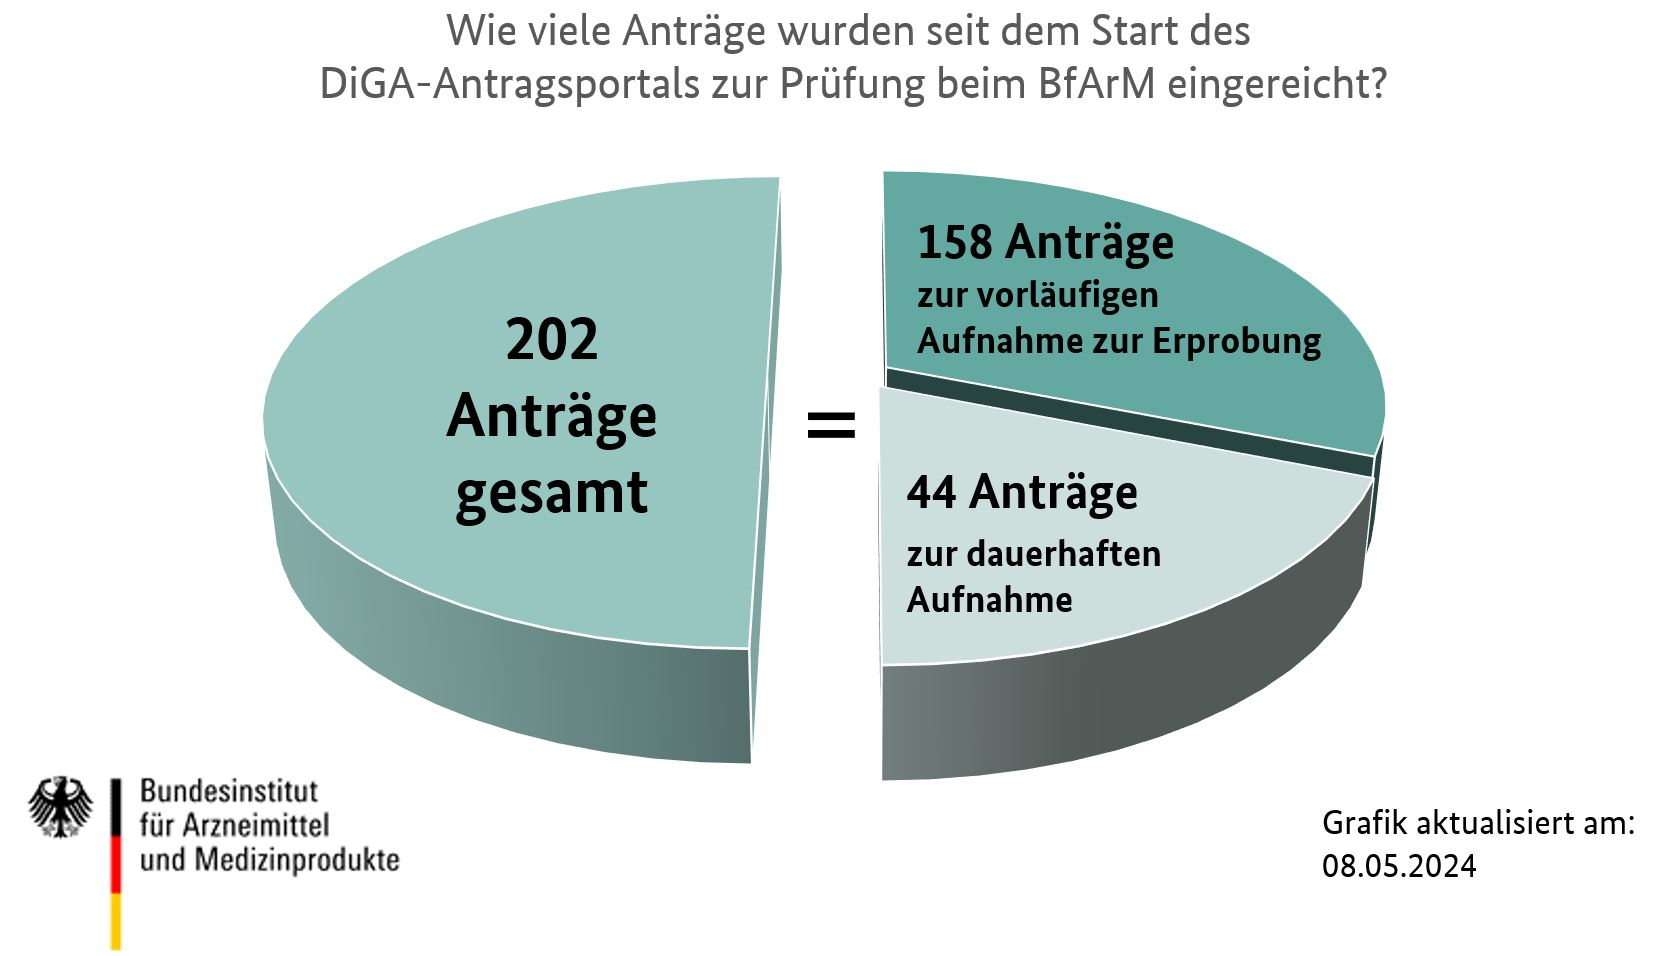
\includegraphics[width=\textwidth]{./grafiken/Anzahl_Antraege_DiGA}
				\caption[Anzahl Anträge von DiGAs]{Kuchendiagramm zur Anzahl von Anträgen von DiGAs}
				\label{Abb-antragsanzahl-diga}
			\end{figure}
			In der Abbildung kann man die Aufteilung der Gesamt Anträge sehen. Von den insgesamt 202 Anträge, wurden 44 Anträge direkt dauerhaft aufgenommen. Daraus kann man schließen das circa 75 Prozent der Anträge, zum Zeitpunkt der Antragsanstellung, noch einen ungewissen medizinischen Nutzen hatten.
			\newpage
			\begin{figure}[htbp]
				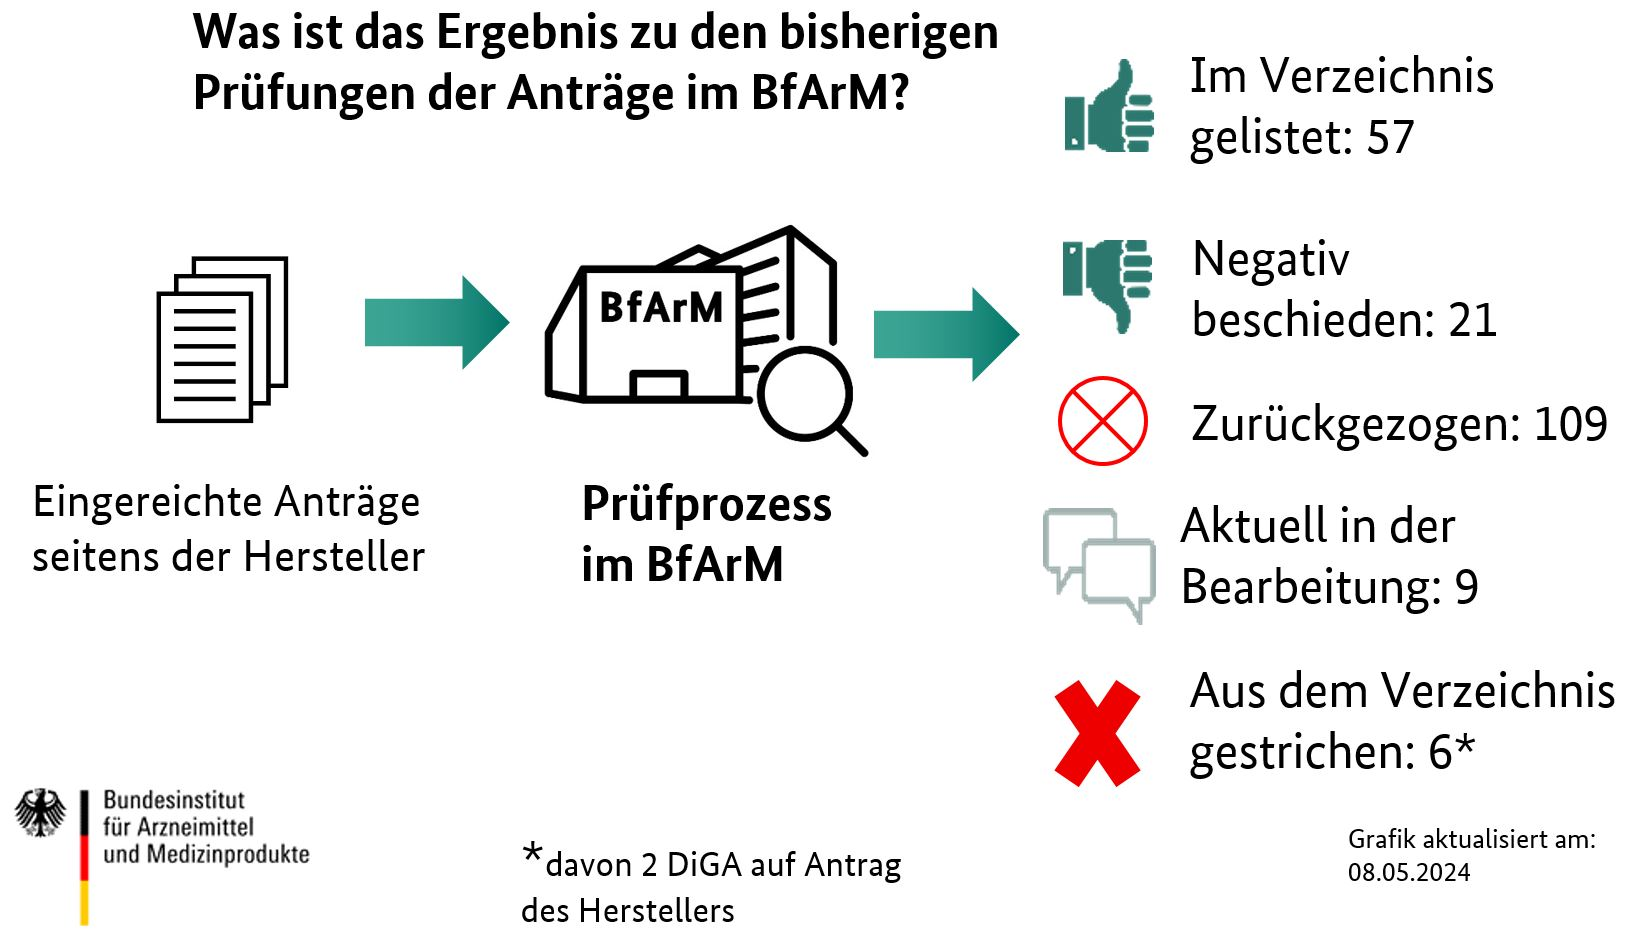
\includegraphics[width=\textwidth]{./grafiken/Ergebnis_Pruefungen_DiGA}
				\caption[Abbildung zu den Ergebnissen des Fast-Track-Verfahren]{Diagramm zu den Ergebnissen des Fast-Track-Verfahren}
				\label{Abb-ergebnisse-ft}
			\end{figure} 
			In der Abbildung kann man die Prüfergebnisse, der Anträge, des BfArM sehen. Von den 202 Anträgen wurden 109 davon zurückgezogen. Somit wurden mehr als 50 Prozent aller Anträge von den Herstellern zurückgezogen. Laut Angaben des BfArM kommt dies durch inhaltlichen Nachbesserungsbedarf bei den Anträgen zustande, denen die Hersteller nicht rechtzeitig nachkommen konnten, aufgrund der kurzen Fristen des Fast-Track-Verfahren\cite[vgl. Z. 37]{tipps-diga-antragsansteller}       

\bibliographystyle{plain}
\bibliography{seminar_arbeit_marcelo}
\end{document}